\subsubsection{UC12 - Logout}\label{UC12}

\begin{figure}[H]
  \centering
  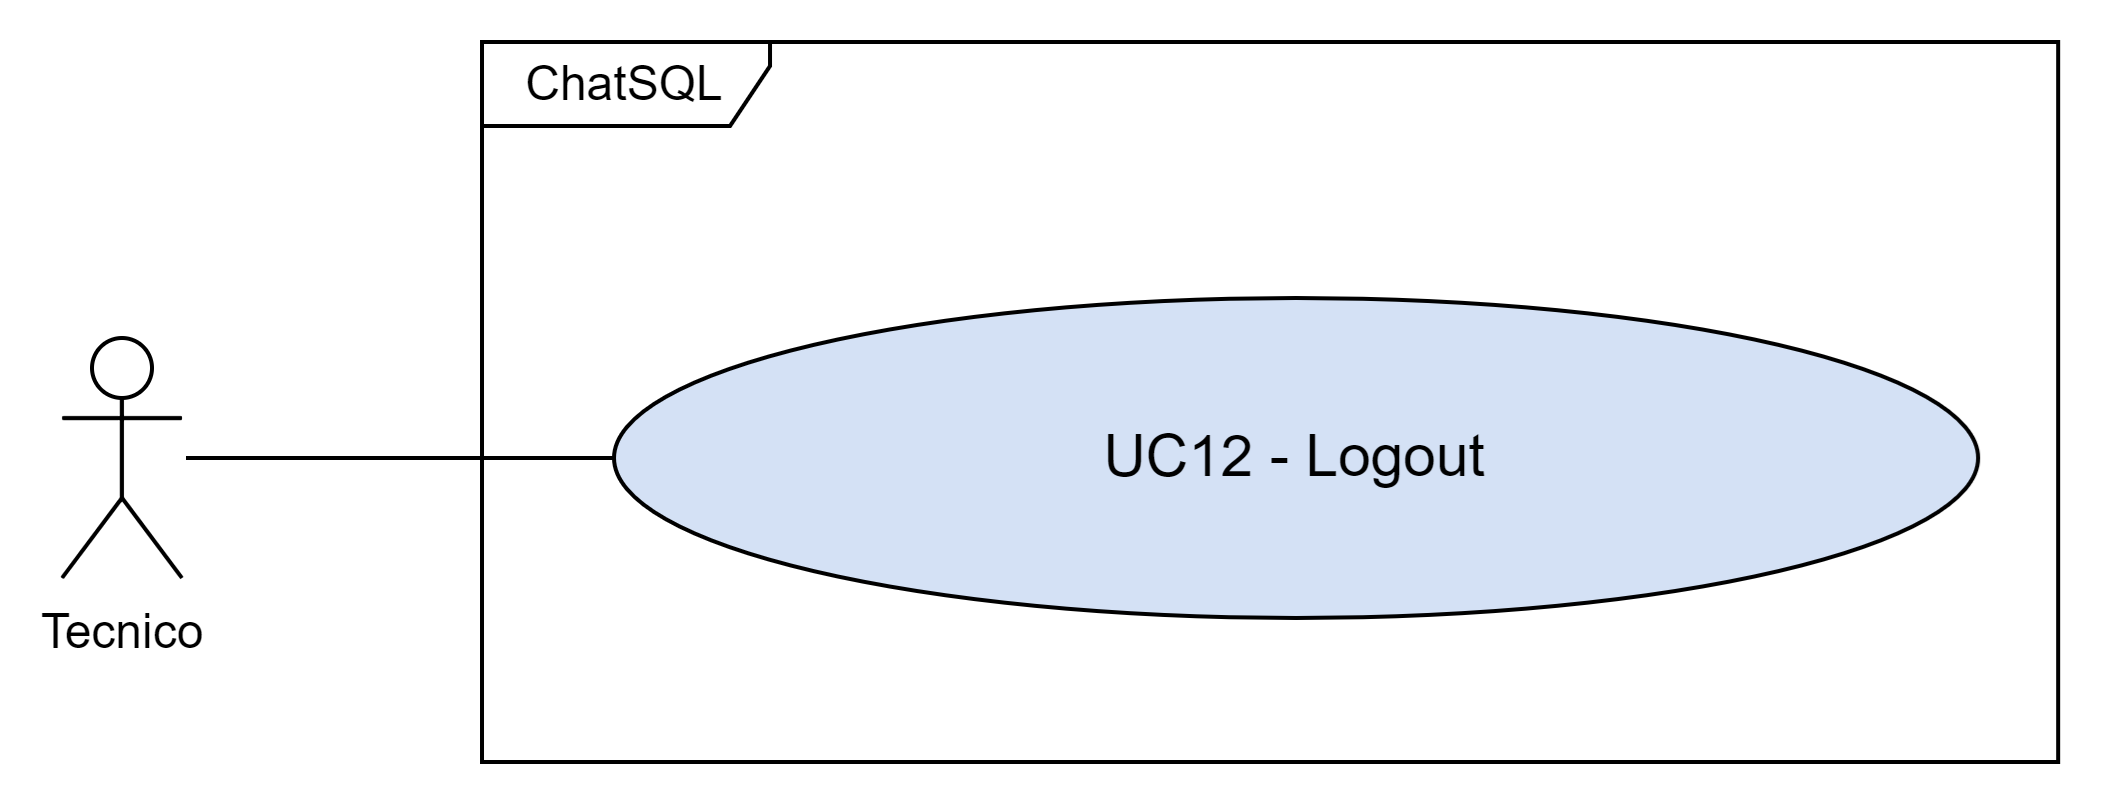
\includegraphics[width=0.90\textwidth]{assets/uc12.png}
  \caption{UC12}
\end{figure}

\paragraph*{Descrizione}
Il logout è una procedura che permette al Tecnico di uscire dall'area e dalle funzionalità che richiedono l'autenticazione.

\paragraph*{Attori principali}
Tecnico

\paragraph*{Precondizioni}
\begin{itemize}
  \item Il Tecnico ha effettuato l'autenticazione (\hyperref[UC1]{UC1}).
\end{itemize}

\paragraph*{Postcondizioni}
\begin{itemize}
  \item Il Tecnico ha eseguito il logout con successo;
  \item Il Tecnico ha a disposizione unicamente le funzionalità che non richiedono l'autenticazione.
\end{itemize}

\paragraph*{Trigger}
Il Tecnico vuole effettuare il logout e terminare la sessione corrente.

\paragraph*{Scenario principale}
\begin{enumerate}
  \item Il Tecnico seleziona l'opzione "Logout";
  \item Viene avviata la procedura di logout;
  \item Il Tecnico viene disconnesso dalla piattaforma.
\end{enumerate}